\documentclass[11pt,a4paper]{report}
\usepackage[textwidth=37em,vmargin=30mm]{geometry}
\usepackage{calc,xunicode,amsmath,amssymb,paralist,enumitem,tabu,booktabs,datetime2,xeCJK,xeCJKfntef,listings}
\usepackage{tocloft,fancyhdr,tcolorbox,xcolor,graphicx,eso-pic,xltxtra,xelatexemoji}

\newcommand{\envyear}[0]{2024}
\newcommand{\envdatestr}[0]{2024-11-20}
\newcommand{\envfinaldir}[0]{webdb/2024/20241120/final}

\usepackage[hidelinks]{hyperref}
\hypersetup{
    colorlinks=false,
    pdfpagemode=FullScreen,
    pdftitle={Web Digest - \envdatestr}
}

\setlength{\cftbeforechapskip}{10pt}
\renewcommand{\cftchapfont}{\rmfamily\bfseries\large\raggedright}
\setlength{\cftbeforesecskip}{2pt}
\renewcommand{\cftsecfont}{\sffamily\small\raggedright}

\setdefaultleftmargin{2em}{2em}{1em}{1em}{1em}{1em}

\usepackage{xeCJK,xeCJKfntef}
\xeCJKsetup{PunctStyle=plain,RubberPunctSkip=false,CJKglue=\strut\hskip 0pt plus 0.1em minus 0.05em,CJKecglue=\strut\hskip 0.22em plus 0.2em}
\XeTeXlinebreaklocale "zh"
\XeTeXlinebreakskip = 0pt


\setmainfont{Brygada 1918}
\setromanfont{Brygada 1918}
\setsansfont{IBM Plex Sans}
\setmonofont{JetBrains Mono NL}
\setCJKmainfont{Noto Serif CJK SC}
\setCJKromanfont{Noto Serif CJK SC}
\setCJKsansfont{Noto Sans CJK SC}
\setCJKmonofont{Noto Sans CJK SC}

\setlength{\parindent}{0pt}
\setlength{\parskip}{8pt}
\linespread{1.15}

\lstset{
	basicstyle=\ttfamily\footnotesize,
	numbersep=5pt,
	backgroundcolor=\color{black!5},
	showspaces=false,
	showstringspaces=false,
	showtabs=false,
	tabsize=2,
	captionpos=b,
	breaklines=true,
	breakatwhitespace=true,
	breakautoindent=true,
	linewidth=\textwidth
}






\newcommand{\coverpic}[2]{
    % argv: itemurl, authorname
    Cover photo by #2~~(\href{#1}{#1})
}
\newcommand{\makeheader}[0]{
    \begin{titlepage}
        % \newgeometry{hmargin=15mm,tmargin=21mm,bmargin=12mm}
        \begin{center}
            
            \rmfamily\scshape
            \fontspec{BaskervilleF}
            \fontspec{Old Standard}
            \fontsize{59pt}{70pt}\selectfont
            WEB\hfill DIGEST
            
            \vfill
            % \vskip 30pt
            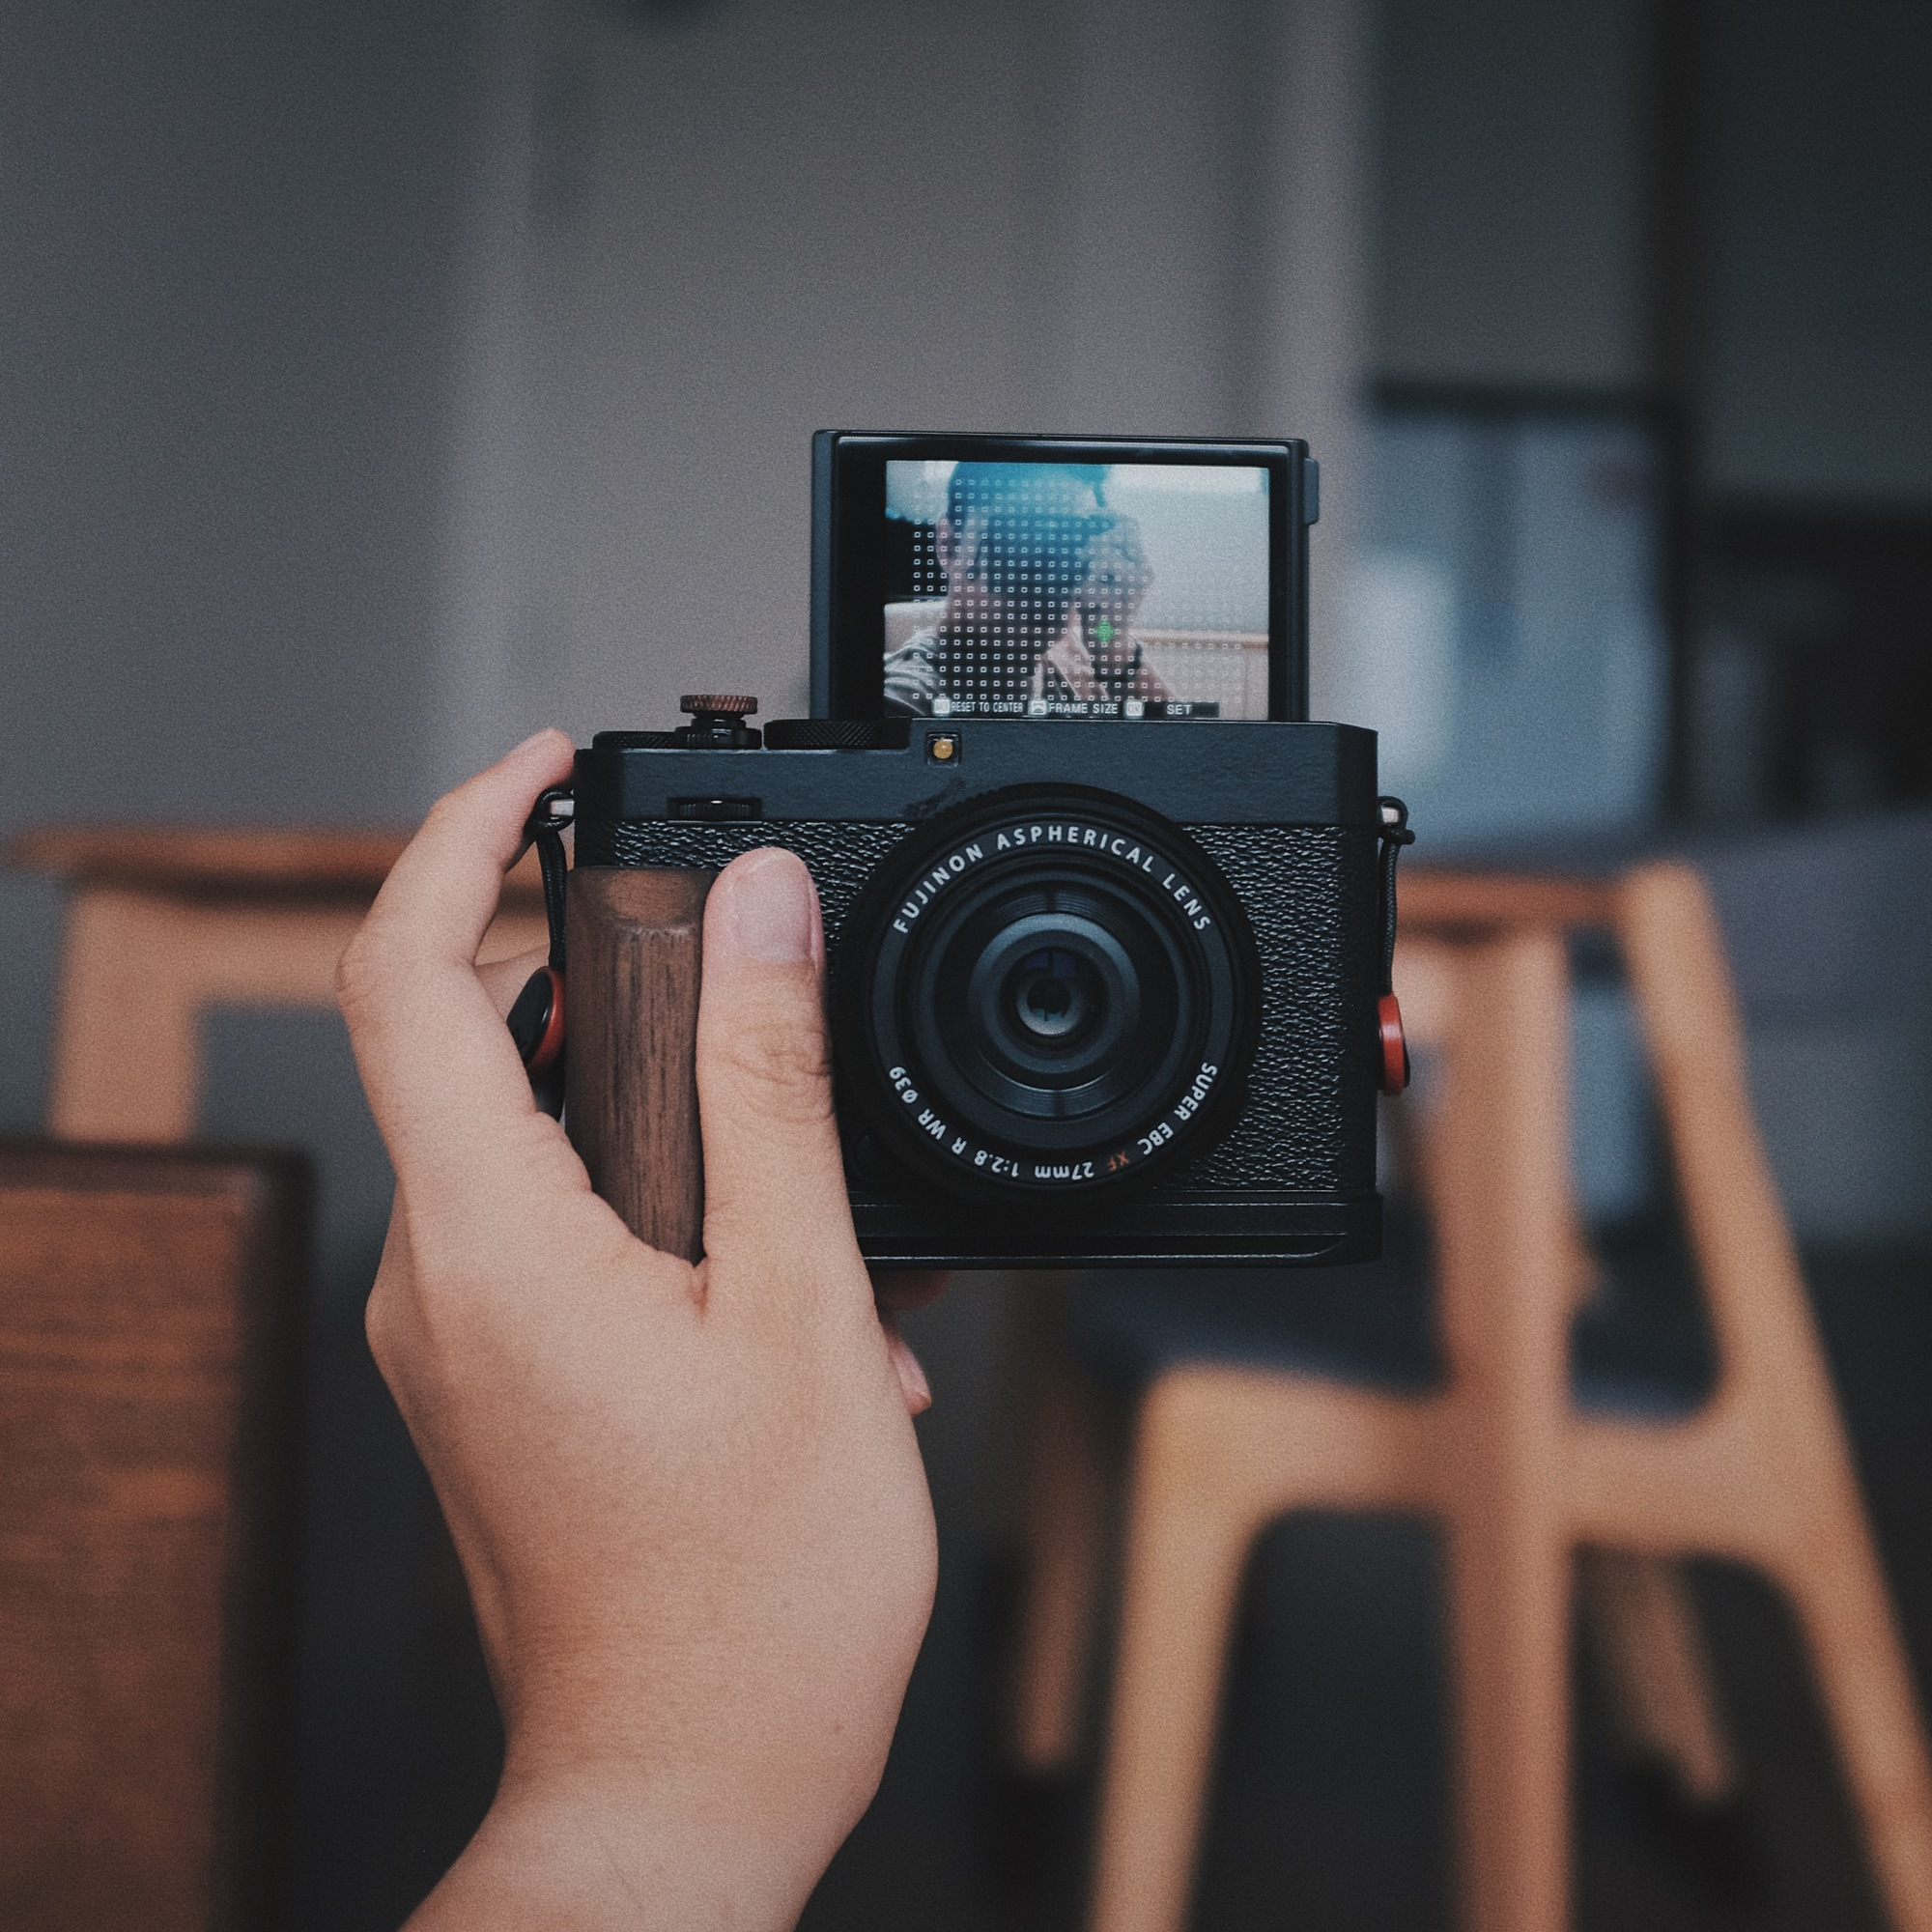
\includegraphics[width=\linewidth]{\envfinaldir/coverpic-prod.jpg}\par
            % \vskip 30pt
            \vfill

            \normalsize\rmfamily\scshape
            \copyright{} The Web Digest Project \hfill\large \envdatestr
        \end{center}
    \end{titlepage}
    % \restoregeometry
}
\newcommand{\simplehref}[1]{%
    \textcolor{blue!80!green}{\href{#1}{#1}}%
}
\renewcommand{\contentsname}{\center\Huge\sffamily\bfseries Contents\par\vskip 20pt}
\newcounter{ipartcounter}
\setcounter{ipartcounter}{0}
\newcommand{\ipart}[1]{
    % \vskip 20pt
    \clearpage
    \stepcounter{ipartcounter}
    \phantomsection
    \addcontentsline{toc}{chapter}{#1}
    % \begin{center}
    %     \Huge
    %     \sffamily\bfseries
    %     #1
    % \end{center}
    % \vskip 20pt plus 7pt
}
\newcounter{ichaptercounter}
\setcounter{ichaptercounter}{0}
\newcommand{\ichapter}[1]{
    % \vskip 20pt
    \clearpage
    \stepcounter{ichaptercounter}
    \phantomsection
    \addcontentsline{toc}{section}{\numberline{\arabic{ichaptercounter}}#1}
    \begin{center}
        \Huge
        \sffamily\bfseries
        #1
    \end{center}
    \vskip 20pt plus 7pt
}
\newcommand{\entrytitlefont}[1]{\subsection*{\raggedright\Large\sffamily\bfseries#1}}
\newcommand{\entryitemGeneric}[2]{
    % argv: title, url
    \parbox{\linewidth}{
        \entrytitlefont{#1}\par\vskip 5pt
        \footnotesize\ttfamily\mdseries
        \simplehref{#2}
    }\vskip 11pt plus 11pt minus 1pt
}
\newcommand{\entryitemGithub}[3]{
    % argv: title, url, desc
    \parbox{\linewidth}{
        \entrytitlefont{#1}\par\vskip 5pt
        \footnotesize\ttfamily\mdseries
        \simplehref{#2}\par\vskip 5pt
        \small\rmfamily\mdseries#3
    }\vskip 11pt plus 11pt minus 1pt
}
\newcommand{\entryitemAp}[3]{
    % argv: title, url, desc
    \parbox{\linewidth}{
        \entrytitlefont{#1}\par\vskip 5pt
        \footnotesize\ttfamily\mdseries
        \simplehref{#2}\par\vskip 5pt
        \small\rmfamily\mdseries#3
    }\vskip 11pt plus 11pt minus 1pt
}
\newcommand{\entryitemHackernews}[3]{
    % argv: title, hnurl, rawurl
    % \parbox{\linewidth}{
    %     \entrytitlefont{#1}\par\vskip 5pt
    %     \footnotesize\ttfamily\mdseries
    %     \simplehref{#3}\par
    %     \textcolor{black!50}{\href{#2}{#2}}
    % }\vskip 11pt plus 11pt minus 1pt
    \begin{minipage}{\linewidth}
            \entrytitlefont{#1}\par\vskip 5pt
            \footnotesize\ttfamily\mdseries
            \simplehref{#3}\par
            \textcolor{black!50}{\href{#2}{#2}}
    \end{minipage}\par\vskip 11pt plus 11pt minus 1pt
}







\begin{document}

\makeheader

\tableofcontents\clearpage




\ipart{Developers}
\ichapter{Hacker News}
\entryitemTwoLinks{Open Riak – open, modern Riak fork}{https://news.ycombinator.com/item?id=42187766}{https://github.com/OpenRiak}

\entryitemTwoLinks{Using Erlang hot code updates}{https://news.ycombinator.com/item?id=42187761}{https://underjord.io/how-i-use-erlang-hot-code-updates.html}

\entryitemTwoLinks{When did estimates turn into deadlines?}{https://news.ycombinator.com/item?id=42187506}{https://domainanalysis.io/p/architecture-modernization-execution}

\entryitemTwoLinks{Hand Tracking for Mouse Input}{https://news.ycombinator.com/item?id=42185842}{https://chernando.com/blog/2023/07/23/hand-tracking-for-mouse-input.html}

\entryitemTwoLinks{Show HN: Physically accurate black hole simulation using your iPhone camera}{https://news.ycombinator.com/item?id=42185668}{https://apps.apple.com/us/app/black-hole-vision/id6737292448}

\entryitemTwoLinks{Shift Left Is the Tip of the Iceberg}{https://news.ycombinator.com/item?id=42183561}{https://semiengineering.com/shift-left-is-the-tip-of-the-iceberg/}

\entryitemTwoLinks{Joint Declaration by Ministers of Germany, France, Poland, Italy, Spain, UK}{https://news.ycombinator.com/item?id=42182897}{https://www.auswaertiges-amt.de/en/newsroom/news/-/2685538}

\entryitemTwoLinks{Show HN: Rust library for numerical integration of real-valued functions}{https://news.ycombinator.com/item?id=42182784}{https://github.com/mtantaoui/Integrate}

\entryitemTwoLinks{OpenStreetMap's New Vector Tiles}{https://news.ycombinator.com/item?id=42182519}{https://tech.marksblogg.com/osm-mvt-vector-tiles.html}

\entryitemTwoLinks{Show HN: Embed an SQLite database in your PostgreSQL table}{https://news.ycombinator.com/item?id=42182146}{https://github.com/frectonz/pglite-fusion}

\entryitemTwoLinks{Listen to what gets lost when an MP3 is made (2015)}{https://news.ycombinator.com/item?id=42181467}{https://www.vox.com/2015/3/4/8147377/mp3-compressed-ghosts}

\entryitemTwoLinks{Fair coins tend to land on the side they started}{https://news.ycombinator.com/item?id=42181345}{https://www.researchgate.net/publication/374700857\_Fair\_coins\_tend\_to\_land\_on\_the\_same\_side\_they\_started\_Evidence\_from\_350757\_flips}

\entryitemTwoLinks{How to Build a Chess Engine and Fail}{https://news.ycombinator.com/item?id=42180597}{https://obrhubr.org/chess-engine}

\entryitemTwoLinks{Rats learned to drive}{https://news.ycombinator.com/item?id=42179774}{https://theconversation.com/im-a-neuroscientist-who-taught-rats-to-drive-their-joy-suggests-how-anticipating-fun-can-enrich-human-life-239029}

\entryitemTwoLinks{Maslow 4: Large format CNC routing made accessible}{https://news.ycombinator.com/item?id=42179467}{https://www.maslowcnc.com}

\entryitemTwoLinks{Why I hate the index finger (1980)}{https://news.ycombinator.com/item?id=42178916}{https://pmc.ncbi.nlm.nih.gov/articles/PMC2997957/}

\entryitemTwoLinks{Llama 3.1 405B now runs at 969 tokens/s on Cerebras Inference}{https://news.ycombinator.com/item?id=42178761}{https://cerebras.ai/blog/llama-405b-inference}

\entryitemTwoLinks{DOJ will push Google to sell off Chrome}{https://news.ycombinator.com/item?id=42177767}{https://www.bloomberg.com/news/articles/2024-11-18/doj-will-push-google-to-sell-off-chrome-to-break-search-monopoly}

\entryitemTwoLinks{Scientific American's departing editor and the politicization of science}{https://news.ycombinator.com/item?id=42177619}{https://reason.com/2024/11/18/how-scientific-americans-departing-editor-helped-degrade-science/}

\entryitemTwoLinks{Hyperfine: A command-line benchmarking tool}{https://news.ycombinator.com/item?id=42177462}{https://github.com/sharkdp/hyperfine}\ichapter{Phoronix}
\entryitemGeneric{\hskip 0pt{}FLTK 1.4 Released With Wayland \& HiDPI Display Support}{https://www.phoronix.com/news/FLTK-1.4-Released}

\entryitemGeneric{\hskip 0pt{}New Linux Patch Lets You Force CPU Bugs/Mitigations Even When Not Vulnerable}{https://www.phoronix.com/news/Linux-force\_cpu\_bug}

\entryitemGeneric{\hskip 0pt{}Blender 4.3 Released With AMD HIP-RT Ray-Tracing On Linux, Experimental Vulkan Backend}{https://www.phoronix.com/news/Blender-4.3-Released}

\entryitemGeneric{\hskip 0pt{}FreeCAD 1.0 Released With UI/UX Improvements, New Materials System}{https://www.phoronix.com/news/FreeCAD-1.0-Released}

\entryitemGeneric{\hskip 0pt{}Linux 6.13 PM Switches EPYC Turin To AMD P-State, More Aggressive Default For Intel GNR}{https://www.phoronix.com/news/Linux-6.13-Power-Management}

\entryitemGeneric{\hskip 0pt{}Red Hat \& Microsoft Bringing RHEL To WSL}{https://www.phoronix.com/news/Red-Hat-MS-RHEL-WSL}

\entryitemGeneric{\hskip 0pt{}Debian 13 Is Quickly Approaching - Desktop Artwork Voting Now Underway}{https://www.phoronix.com/news/Debian-13-Trixie-Artwork-Survey}

\entryitemGeneric{\hskip 0pt{}WayVNC 0.9 Released For Wayland VNC Server With New Features}{https://www.phoronix.com/news/WayVNC-0.9-Wayland-VNC}

\entryitemGeneric{\hskip 0pt{}MiTAC Releases AMD openSIL Based Open-Source Firmware For Their Capri2 EPYC Server}{https://www.phoronix.com/news/MiTAC-Capri2-OpenSIL-Firmware}


\ipart{Developers~~~~(zh-Hans)}
\ichapter{Solidot}
\entryitemGeneric{\hskip 0pt{}恐龙时代的鸟脑化石填补了鸟脑演化的空白}{https://www.solidot.org/story?sid=79823}

\entryitemGeneric{\hskip 0pt{}中国启动世界最大超重力实验装置}{https://www.solidot.org/story?sid=79822}

\entryitemGeneric{\hskip 0pt{}科学家发现耐药菌的致命弱点}{https://www.solidot.org/story?sid=79821}

\entryitemGeneric{\hskip 0pt{}哈珀柯林斯证实出售部分非虚构作品用于 AI 训练}{https://www.solidot.org/story?sid=79820}

\entryitemGeneric{\hskip 0pt{}中国人口未来十年预计将减少 5100 万}{https://www.solidot.org/story?sid=79819}

\entryitemGeneric{\hskip 0pt{}减肥药诺和盈在中国上市}{https://www.solidot.org/story?sid=79818}

\entryitemGeneric{\hskip 0pt{}使用互联网可能有助于提升 50 岁以上人群幸福感}{https://www.solidot.org/story?sid=79817}

\entryitemGeneric{\hskip 0pt{}微软在东京设立日本首个研究基地}{https://www.solidot.org/story?sid=79816}

\entryitemGeneric{\hskip 0pt{}AlmaLinux 9.5 释出}{https://www.solidot.org/story?sid=79815}

\entryitemGeneric{\hskip 0pt{}Google 将杀死 Chrome OS}{https://www.solidot.org/story?sid=79814}

\entryitemGeneric{\hskip 0pt{}El Capitan 登顶 Top500 超算榜单}{https://www.solidot.org/story?sid=79813}

\entryitemGeneric{\hskip 0pt{}Valve 开发者解释为什么取消开发《半条命 2:第三章》}{https://www.solidot.org/story?sid=79812}

\entryitemGeneric{\hskip 0pt{}美国司法部将推动 Google 出售 Chrome}{https://www.solidot.org/story?sid=79811}

\entryitemGeneric{\hskip 0pt{}蒂姆·伯纳斯-李想要互联网回归自由民主}{https://www.solidot.org/story?sid=79810}

\entryitemGeneric{\hskip 0pt{}华盛顿州圣胡安县推行 32 小时工作制一周年}{https://www.solidot.org/story?sid=79809}

\entryitemGeneric{\hskip 0pt{}中国温室气体排放继续缓慢增长,美国下降}{https://www.solidot.org/story?sid=79808}

\entryitemGeneric{\hskip 0pt{}空气污染与湿疹存在相关性}{https://www.solidot.org/story?sid=79807}

\entryitemGeneric{\hskip 0pt{}中国在珠海航展上展示可重复使用的昊龙货运航天飞机}{https://www.solidot.org/story?sid=79806}

\entryitemGeneric{\hskip 0pt{}微软释出 Windows 11 for Arm 镜像下载}{https://www.solidot.org/story?sid=79805}

\entryitemGeneric{\hskip 0pt{}研究发现 X 算法偏爱共和党和马斯克}{https://www.solidot.org/story?sid=79804}\ichapter{V2EX}
\entryitemGeneric{\hskip 0pt{}[iPadOS] 突然发现 iPadOS 邮件 app 一个有趣的功能,双击项目可以在小窗打开,再点击小窗外空白处可以进入多窗口模式~}{https://www.v2ex.com/t/1091014}

\entryitemGeneric{\hskip 0pt{}[Go 编程语言] 分享开源项目 Passport,一行 URL 搞定可信认证、网络穿透和端口转发}{https://www.v2ex.com/t/1091012}

\entryitemGeneric{\hskip 0pt{}[互联网] [help] 请大神帮忙下看 clash meta 的配置哪里有问题,谢谢}{https://www.v2ex.com/t/1091011}

\entryitemGeneric{\hskip 0pt{}[问与答] 求助: WIN10 96G 内存被吃满, poolmon 和 RamMap 都找不出凶手}{https://www.v2ex.com/t/1091010}

\entryitemGeneric{\hskip 0pt{}[iOS] Tampermonkey 终于空降 iOS}{https://www.v2ex.com/t/1091009}

\entryitemGeneric{\hskip 0pt{}[.NET] Avalonia 11 后要从 ItemsControl 调用母 UserControl 的命令这种常见操作就必须每次都写这么长一坨东西吗?}{https://www.v2ex.com/t/1091008}

\entryitemGeneric{\hskip 0pt{}[宜家] 求大家分享一下用过的淘宝宜家代购店铺?}{https://www.v2ex.com/t/1091007}

\entryitemGeneric{\hskip 0pt{}[分享创造] 如何避免被同行发现你的产品?一起分享一下如何避免被同行发现你的产品?更好的绕过同行接触到用户🤔}{https://www.v2ex.com/t/1091006}

\entryitemGeneric{\hskip 0pt{}[程序员] 有开发者吗 满足一下好奇心。}{https://www.v2ex.com/t/1091004}

\entryitemGeneric{\hskip 0pt{}[OpenAI] 大家现在工作中更喜欢 claude 还是 chatgpt?}{https://www.v2ex.com/t/1091003}

\entryitemGeneric{\hskip 0pt{}[推广] [飞猪推广]度假错峰游,门票 5 折起}{https://www.v2ex.com/t/1091001}

\entryitemGeneric{\hskip 0pt{}[程序员] 使用 cloudflare 前端站点出现加载不到资源文件}{https://www.v2ex.com/t/1090999}

\entryitemGeneric{\hskip 0pt{}[宽带症候群] 新版 sunshine 被河北联通 5G 网智能阻断?}{https://www.v2ex.com/t/1090997}

\entryitemGeneric{\hskip 0pt{}[分享创造] 带 Web UI 的开源堡垒机,支持 RDP、VNC、SSH 远程桌面、主机、数据库、文件管理、内网穿透、批量执行命令、远程 OS 升级}{https://www.v2ex.com/t/1090996}

\entryitemGeneric{\hskip 0pt{}[程序员] 现代化 SSH 客户端求推荐}{https://www.v2ex.com/t/1090995}

\entryitemGeneric{\hskip 0pt{}[问与答] 某铺子为什么没有知情人发声?}{https://www.v2ex.com/t/1090992}

\entryitemGeneric{\hskip 0pt{}[程序员] 非专职开发让 AI 帮你写出无 bug 的代码的一些心得}{https://www.v2ex.com/t/1090990}

\entryitemGeneric{\hskip 0pt{}[香港] 请问黑五在香港买果机 16 有折扣吗,折扣大概多大}{https://www.v2ex.com/t/1090989}

\entryitemGeneric{\hskip 0pt{}[Apple] 国区账号加入美区 Apple One 的家庭分享,能用哪几项服务?}{https://www.v2ex.com/t/1090988}

\entryitemGeneric{\hskip 0pt{}[推广] 飞行员刷题神器,想到处飞的朋友有福了}{https://www.v2ex.com/t/1090987}

\entryitemGeneric{\hskip 0pt{}[iOS] 在另一个论坛看到 iOS 的源阅读,可以付费购买 TestFlight 资格,哪位大哥知道购买途径的?}{https://www.v2ex.com/t/1090986}

\entryitemGeneric{\hskip 0pt{}[NAS] jellyfin docker 突然无法启动}{https://www.v2ex.com/t/1090985}

\entryitemGeneric{\hskip 0pt{}[问与答] github 号没了怎么办??急急急}{https://www.v2ex.com/t/1090984}

\entryitemGeneric{\hskip 0pt{}[分享发现] Cursor 还有哪些意想不到的惊喜?}{https://www.v2ex.com/t/1090983}

\entryitemGeneric{\hskip 0pt{}[Apple] 一些 Apple 设备的问题,想请教大家是否有解}{https://www.v2ex.com/t/1090980}

\entryitemGeneric{\hskip 0pt{}[创业组队] Allin 提升人类生产力!有想创业的技术伙伴欢迎来找我~}{https://www.v2ex.com/t/1090979}

\entryitemGeneric{\hskip 0pt{}[问与答] 各位 v 友有没有吃瓜飞机群推荐呢?}{https://www.v2ex.com/t/1090978}

\entryitemGeneric{\hskip 0pt{}[分享创造] RIME 配置和词库集「雾凇拼音」还差几百就到 10k star 了,来随便聊聊宣传下}{https://www.v2ex.com/t/1090977}

\entryitemGeneric{\hskip 0pt{}[问与答] 看很多都在买 racknerds 的黑五主机,它的作用是啥,用来搭梯子还是别的看不到的好处}{https://www.v2ex.com/t/1090975}

\entryitemGeneric{\hskip 0pt{}[Apple] 有什么办法隐藏 dock 栏用不上的图标(qq,微信)}{https://www.v2ex.com/t/1090974}

\entryitemGeneric{\hskip 0pt{}[问与答] 有没有什么能部署在网关,拦截各大 App 的 PCDN 业务的解决方案?就类似 Adguard Home 拦截广告的感觉一样?}{https://www.v2ex.com/t/1090973}

\entryitemGeneric{\hskip 0pt{}[宽带症候群] 现在拨号上网获得的 IP 都是同一个网段不会变了吗?}{https://www.v2ex.com/t/1090970}

\entryitemGeneric{\hskip 0pt{}[问与答] 被骗了,但是拿对方毫无办法}{https://www.v2ex.com/t/1090969}

\entryitemGeneric{\hskip 0pt{}[程序员] 新手程序员求助,关于如何提取.cpp 内的代码和注释。}{https://www.v2ex.com/t/1090968}

\entryitemGeneric{\hskip 0pt{}[VPS] VPS 适合挂博客吗?}{https://www.v2ex.com/t/1090967}

\entryitemGeneric{\hskip 0pt{}[问与答] 这个银行信息怎么填呢?}{https://www.v2ex.com/t/1090966}

\entryitemGeneric{\hskip 0pt{}[硬件] 手上有个兄弟打印机激光的,但是需要链接电脑才能使用}{https://www.v2ex.com/t/1090965}

\entryitemGeneric{\hskip 0pt{}[问与答] 请教 V 友是否有合适的工具,可以让业余人家进行 web 和 app 端的产品和 UI 设计}{https://www.v2ex.com/t/1090964}

\entryitemGeneric{\hskip 0pt{}[支付宝] 我也来吐槽一下支付宝}{https://www.v2ex.com/t/1090963}

\entryitemGeneric{\hskip 0pt{}[分享发现] 黑龙江 365 流量卡办理教程(永久套餐 共享 支持副卡 VVIP 速率 )}{https://www.v2ex.com/t/1090962}

\entryitemGeneric{\hskip 0pt{}[阅读] 微信读书自动打卡刷时长}{https://www.v2ex.com/t/1090961}

\entryitemGeneric{\hskip 0pt{}[Apple] 求科普,苹果 M 芯片的编解码引擎,作用在视频剪辑哪里❓}{https://www.v2ex.com/t/1090960}

\entryitemGeneric{\hskip 0pt{}[全球工单系统] 有微信做人脸识别的兄弟吗? Pixel 8 的前置摄像头预览界面有广角,人脸识别用不了}{https://www.v2ex.com/t/1090959}

\entryitemGeneric{\hskip 0pt{}[互联网] 请教 v 站有从事第三方支付、清算业务相关的大佬吗,这行的业务如何去了解?}{https://www.v2ex.com/t/1090957}

\entryitemGeneric{\hskip 0pt{}[Android] 谁能帮我写个安卓 app,显示电池百分比的悬浮窗,您可以在下拉的 quick setting 中有开关。}{https://www.v2ex.com/t/1090956}

\entryitemGeneric{\hskip 0pt{}[问与答] windows 如何找出某个域名是哪个程序在试图访问?}{https://www.v2ex.com/t/1090955}

\entryitemGeneric{\hskip 0pt{}[问与答] 入手了一个群晖 nas 224,求系列的教程~}{https://www.v2ex.com/t/1090954}

\entryitemGeneric{\hskip 0pt{}[支付宝] 我也吐槽下遇到的支付宝 Bug}{https://www.v2ex.com/t/1090951}

\entryitemGeneric{\hskip 0pt{}[问与答] 问下各位用 mac 的,请问怎么单击 dock 栏上的图标 打开和最小化软件?}{https://www.v2ex.com/t/1090950}

\entryitemGeneric{\hskip 0pt{}[Excel] 单元格内数据去重 纯分享 解决工作难题}{https://www.v2ex.com/t/1090949}


\ipart{Generic News}
\ichapter{AP News}
\entryitemWithDescription{\hskip 0pt{}An emotional Rafael Nadal retires at the Davis Cup after he loses and Spain is eliminated}{https://apnews.com/article/540a85d63be118e74aa29cacee927e04}{}

\entryitemWithDescription{\hskip 0pt{}Bruins fire coach Jim Montgomery after slow start in regular season follows playoff disappointments}{https://apnews.com/article/0dcb944f383eb2652a4ae5e7549854ca}{}

\entryitemWithDescription{\hskip 0pt{}Italy recovers Etruscan artifacts worth \$8.5 million bound for black market}{https://apnews.com/article/d74656945ceecdbbbfcedfdb51944bce}{}

\entryitemWithDescription{\hskip 0pt{}4 monkeys remain free nearly 2 weeks after dozens escaped a South Carolina compound}{https://apnews.com/article/9055f3163378ff2aa821f6d2e8f8c0f1}{}

\entryitemWithDescription{\hskip 0pt{}Shaun White's new halfpipe league to air on NBC, Peacock}{https://apnews.com/article/36c274691cf5cc76e4709b35ce5f3600}{}

\entryitemWithDescription{\hskip 0pt{}Romanian court finds irregularities in prosecutors' case against Andrew Tate}{https://apnews.com/article/8e1f78567334ae2ae5f2ae63855d218a}{}

\entryitemWithDescription{\hskip 0pt{}51-year-old man is charged with murder after 3 are stabbed in New York City rampage}{https://apnews.com/article/839937c4da562c1a7ac51a0cb1cd58db}{}

\entryitemWithDescription{\hskip 0pt{}Jersey Mike's sandwich chain is acquired by private equity firm Blackstone for \$8 billion}{https://apnews.com/article/d45eb865f912eb39bbd7ac8ad8a86fcd}{}

\entryitemWithDescription{\hskip 0pt{}New Harry Potter ride at Universal Orlando will have British Ministry of Magic as setting}{https://apnews.com/article/b0f0c95c34948fc1b4ca5c19e8e668eb}{}

\entryitemWithDescription{\hskip 0pt{}The White House's Christmas tree is a symbol of resilience for hurricane-hit North Carolina farms}{https://apnews.com/article/e4868d6b13c65cd4944c5fe26fafb058}{}

\entryitemWithDescription{\hskip 0pt{}School closures and travel delays as Arctic air brings snow and sleet to parts of the UK}{https://apnews.com/article/e782cedaf45b4ee24fc5c489637e0461}{}

\entryitemWithDescription{\hskip 0pt{}Texans never trail while handing Cowboys 5th straight loss, 34-10}{https://apnews.com/article/22aa2f02bb1505593491b07238e320a0}{}

\entryitemWithDescription{\hskip 0pt{}Arthur Frommer, travel guide innovator, has died at 95}{https://apnews.com/article/7293814296854079a3a10f05d02faf44}{}\ichapter{Reuters}
\entryitemWithDescription{\hskip 0pt{}Speak up against Band Aid Christmas hit, British-Ghanaian singer tells music stars}{https://www.reuters.com/world/speak-up-against-band-aid-christmas-hit-british-ghanaian-singer-tells-music-2024-11-19/}{British-Ghanaian musician Fuse ODG has urged other artists to follow in the steps of Ed Sheeran and speak up about the 1984 hit "Do They Know It\textquotesingle s Christmas," which he says perpetuates negative stereotypes of the African...}

\entryitemWithDescription{\hskip 0pt{}Trump administration plans to roll back Biden's stricter fuel-efficiency standards}{https://www.reuters.com/world/us/trump-administration-plans-roll-back-bidens-stricter-fuel-efficiency-standards-2024-11-19/}{President-elect Donald Trump\textquotesingle s incoming administration plans to target federal regulations championed by President Joe Biden that aim to make automobiles more fuel-efficient and incentivize a shift toward electric...}

\entryitemWithDescription{\hskip 0pt{}Russian air defences down Ukrainian drones in six regions}{https://www.reuters.com/world/europe/russian-air-defences-down-ukrainian-drones-six-regions-2024-11-19/}{Russian air defence units intercepted Ukrainian drones in six southern and central regions late on Monday, with some damage reported on the ground, but no casualties, officials...}

\entryitemWithDescription{\hskip 0pt{}US State Dept OKs potential sale of F-15 aircraft upgrade to South Korea, Pentagon says}{https://www.reuters.com/world/us-state-dept-oks-potential-sale-f-15-aircraft-upgrade-to-south-korea-pentagon-2024-11-19/}{U.S. State Department has approved the potential sale of F-15K aircraft upgrade and related equipment to South Korea for an estimated cost of \$6.2 billion, the Pentagon said on...}

\entryitemWithDescription{\hskip 0pt{}US State Dept. OKs potential \$100 mln sale of military equipment to Ukraine}{https://www.reuters.com/world/us-state-dept-oks-potential-100-mln-sale-military-equipment-ukraine-2024-11-19/}{The U.S. Department of State has approved the potential \$100 million sale of military equipment and services to Ukraine, the Pentagon said in a statement on...}

\entryitemWithDescription{\hskip 0pt{}Lawsuits allege Colorado officials ignored 'red flag' laws before Club Q shooting}{https://www.reuters.com/legal/lawsuits-allege-colorado-officials-ignored-red-flag-laws-before-club-q-shooting-2024-11-19/}{Victims of a deadly 2022 shooting attack on a gay nightclub in Colorado have sued local authorities, accusing them of failing to enforce a red flag gun law they say could have prevented the...}

\entryitemWithDescription{\hskip 0pt{}Lula cuts G20 discussion short on Ukraine, irking Europeans}{https://www.reuters.com/world/lula-cuts-g20-discussion-short-ukraine-irking-europeans-2024-11-19/}{European delegates at the G20 summit in Brazil were unhappy with President Luiz Inacio Lula da Silva\textquotesingle s decision to end talks and issue the group\textquotesingle s final statement a day early to curtail prickly discussion...}

\entryitemWithDescription{\hskip 0pt{}US, Israeli officials will discuss civilian harm in Gaza in early December, State Department says}{https://www.reuters.com/world/us-israeli-officials-will-discuss-civilian-harm-gaza-early-december-state-2024-11-19/}{Senior U.S. and Israeli officials will hold talks in early December in the first meeting of a new channel requested by Washington to raise concerns over civilian harm in Israel\textquotesingle s war in Gaza, State Department spokesperson...}

\entryitemWithDescription{\hskip 0pt{}Argentina's Milei plays Trump stand-in at G20 summit in Rio}{https://www.reuters.com/world/argentinas-milei-plays-trump-stand-in-g20-summit-rio-2024-11-19/}{As world leaders at the G20 summit in Brazil are bracing for the return of U.S. President Donald Trump to the center of global affairs, one head of state in the room has given them an early taste of a familiar, iconoclastic right-wing...}

\entryitemWithDescription{\hskip 0pt{}Liam Payne's funeral to take place on Wednesday, British media reports}{https://www.reuters.com/world/uk/liam-paynes-funeral-take-place-wednesday-british-media-reports-2024-11-19/}{The funeral of former One Direction star Liam Payne, who died last month in a fall from the balcony of his Buenos Aires, is expected to take place on Wednesday, British media...}

\entryitemWithDescription{\hskip 0pt{}Australia, Turkey in 2026 UN climate summit hosting standoff}{https://www.reuters.com/business/environment/australia-turkey-2026-un-climate-summit-hosting-standoff-2024-11-19/}{Australia and Turkey are in a standoff over which country is better suited to host United Nations climate change talks in 2026, with neither willing to give up on their...}

\entryitemWithDescription{\hskip 0pt{}Netanyahu, in Gaza, says Hamas will no longer rule enclave}{https://www.reuters.com/world/middle-east/netanyahu-gaza-says-hamas-will-no-longer-rule-enclave-2024-11-19/}{Israeli Prime Minister Benjamin Netanyahu said during a visit to Gaza on Tuesday that Hamas would not rule the Palestinian enclave after the war had ended and that Israel had destroyed the Islamist group\textquotesingle s military...}

\entryitemWithDescription{\hskip 0pt{}French farmers continue protests as union threatens food supply disruption}{https://www.reuters.com/world/europe/french-farmers-continue-protests-union-threatens-food-supply-disruption-2024-11-19/}{French farmers held a second day of protests on Tuesday over EU-Mercosur trade talks, with the hardline Coordination Rurale union dumping Spanish wine and blocking official buildings as a prelude to threatened disruption to food supply...}






\clearpage
\leavevmode\vfill
\footnotesize

Copyright \copyright{} 2023-2024 Neruthes and other contributors.

This document is published with CC BY-NC-ND 4.0 license.

The entries listed in this newsletter may be copyrighted by their respective creators.

This newsletter is generated by the Web Digest project.

The newsletters are also delivered via Telegram channel \CJKunderline{\href{https://t.me/webdigestchannel}{https://t.me/webdigestchannel}}.\\
RSS feed is available at \CJKunderline{\href{https://webdigest.pages.dev/rss.xml}{https://webdigest.pages.dev/rss.xml}}.

This newsletter is available in PDF at
\CJKunderline{\href{https://webdigest.pages.dev/}{https://webdigest.pages.dev/}}.

The source code being used to generate this newsletter is available at\\
\CJKunderline{\href{https://github.com/neruthes/webdigest}{https://github.com/neruthes/webdigest}}.

This newsletter is also available in
\CJKunderline{\href{http://webdigest.pages.dev/readhtml/\envyear/WebDigest-20241120.html}{HTML}} and
\CJKunderline{\href{https://github.com/neruthes/webdigest/blob/master/markdown/\envyear/WebDigest-20241120.md}{Markdown}}.


\coverpic{https://unsplash.com/photos/a-foggy-night-with-trees-in-the-distance-2XKR-38TxbU}{Daniil Silantev}


\end{document}
